\begin{figure}[tbp]
\centering
\begin{tikzpicture}
  \node[inner sep=0, anchor=south west] (moon) at (0,0)
    {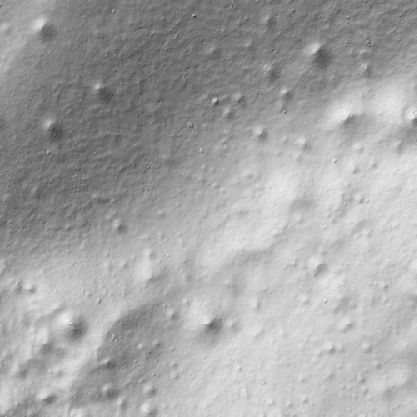
\includegraphics[width=0.42\linewidth]{figures/generated/hillshade-moon.pdf}};
  \node[inner sep=0, anchor=south west] (earth) at ([xshift=0.06\linewidth]moon.south east)
    {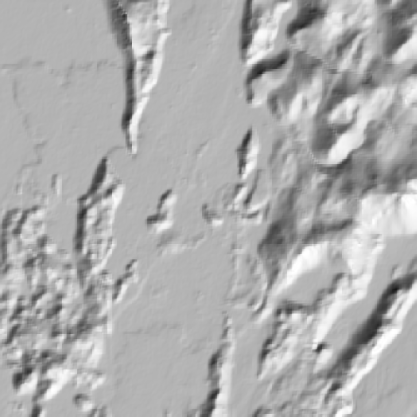
\includegraphics[width=0.42\linewidth]{figures/generated/hillshade-earth.pdf}};
  \foreach \panel in {moon, earth} {
    \draw[line width=0.4pt] (\panel.south west) rectangle (\panel.north east);
    \fill[white, opacity=0.8] ([xshift=4pt, yshift=4pt]\panel.south west)
      rectangle ([xshift={4pt+0.084\linewidth+6pt}, yshift=17pt]\panel.south west);
    \draw[line width=1.2pt] ([xshift=7pt, yshift=8pt]\panel.south west)
      -- ([xshift={7pt+0.084\linewidth}, yshift=8pt]\panel.south west);
    \node[font=\footnotesize, anchor=south] at ([xshift={7pt+0.042\linewidth}, yshift=8pt]\panel.south west) {1 km};
    \draw[-{Stealth[length=4pt]}, line width=0.6pt] ([xshift=-9pt, yshift=-22pt]\panel.north east)
      -- ([xshift=-9pt, yshift=-6pt]\panel.north east);
  }
  \node[font=\footnotesize, anchor=north] at ([xshift=-9pt, yshift=-22pt]moon.north east) {$+y$};
  \node[font=\footnotesize, anchor=north] at ([xshift=-9pt, yshift=-22pt]earth.north east) {N};
  \node[font=\footnotesize, anchor=north] at ([yshift=-2pt]moon.south) {(a) Moon, Connecting Ridge target window};
  \node[font=\footnotesize, anchor=north] at ([yshift=-2pt]earth.south) {(b) Earth, shortlisted Holuhraun window};
\end{tikzpicture}
\caption{Hillshades of the lunar target window and the shortlisted Earth window, each
\ConfigWindowM\,m wide, lit from azimuth \HillAzimuth{} degrees at \HillAltitude{} degrees altitude with no vertical
exaggeration. (a) Window \texttt{moon-sps-x2-y2}, centred at latitude \HillMoonLat{} and longitude \HillMoonLon{}
degrees, from the 5 m surface heights of PGDA product 78 Site01 \citep{barker2021}, shown at every
second pixel in the product's south polar stereographic grid; the arrow is grid north ($+y$). Most
5 m pixels are interpolated between LOLA tracks (Section~\ref{sec:data}). (b) Window
\texttt{earth-utm27n-e285-n2879}, centred at latitude \HillEarthLat{} and longitude \HillEarthLon{} degrees, resampled
from Copernicus GLO-30 tile N64 W017 \citep{airbus2022copernicus} onto a 10 m grid about its centre
with the window resampler; the arrow is north. Generated by \texttt{paper/scripts/figures.py},
which records the input digests.}
\label{fig:hillshades}
\end{figure}
